\documentclass[12pt,twoside,book]{article}
\usepackage{docmute}

\input{../settings}

\begin{document}

%%%%%%%%%%%%%%%%%%%%%%%%%%%%%%%%%%%%%%%%%%%%%%%%%%%%%%%%%%%%%%%%%%%%%%%%%%%%%%%
\section{WIMP as a dark matter}
\setcounter{equation}{0}
\label{sec:DM}
%%%%%%%%%%%%%%%%%%%%%%%%%%%%%%%%%%%%%%%%%%%%%%%%%%%%%%%%%%%%%%%%%%%%%%%%%%%%%%%

\vskip 0.1in

In this section, we review the properties of WIMPs as DM candidates.
It is revealed that, when we take a close look at the relic abundance of WIMP DM in Sec.~\ref{sec:relic}, a WIMP with the $\mathrm{TeV}$ scale mass is a good DM candidate, which is sometimes called \textit{WIMP miracle} and is a strong motivation to consider WIMPs.
In Sec.~\ref{sec:direct_detection} and Sec.~\ref{sec:indirect_detection}, we will consider two different ways to search for WIMP DM, called the direct and indirect detection.
Finally, Sec.~\ref{sec:summary_DM} is devoted to the summary and concluding remarks of this section.


%%%%%%%%%%%%%%%%%%%%%%%%%%%%%%%%%%%%%%%%%%%%%%%%%%%%%%%%%%%%%%%%%%%%%%%%%%%%%%%
\subsection{WIMP DM relic abundance}
\label{sec:relic}
%%%%%%%%%%%%%%%%%%%%%%%%%%%%%%%%%%%%%%%%%%%%%%%%%%%%%%%%%%%%%%%%%%%%%%%%%%%%%%%

One of the most important evidence of the beyond SM phenomena is the existence of DM \cite{Zwicky:1933}.
DM is an unknown object that occupies a large fraction of the total energy of our universe but has not yet been directly observed because of its weak interaction with the SM particles.\footnote{
  At worst DM interacts with the SM particles through gravity, which is considerably weaker than all the other known interactions.
}
In spite of its invisibility, the existence of DM is confirmed by several astrophysical observations such as the mass measurement using the gravitational lensing effect caused by galaxies and clusters \cite{Zwicky:1937, Trimble:1987ee}, the flatness of galactic rotation curves beyond the optical radius \cite{1939LicOB..19...41B, Begeman:1991iy}, the measurement of the power spectrum of the cosmic microwave background (CMB), and so on.
In particular, the observation of CMB allows us the precise determination of various cosmological parameters \cite{Jungman:1995av, Jungman:1995bz} including the normalized density of the non-relativistic matter $\Omega_m$ and that of baryon $\Omega_b$, which is currently determined as \cite{Aghanim:2018eyx}
\begin{align}
  \Omega_m h^2 &= 0.1430 \pm 0.0011,\\
  \Omega_b h^2 &= 0.02237 \pm 0.00015,
\end{align}
where $h \sim 0.7$ is the Hubble constant in units of $100\, \mathrm{km}\, \mathrm{s}^{-1}\, \mathrm{Mpc}^{-1}$.
The difference between $\Omega_m h^2$ and $\Omega_b h^2$ implies the existence of DM and its abundance $\Omega_\chi h^2 \simeq 0.12$.

In cosmology, DM production mechanisms that explain the DM abundance are divided into two large categories: thermal and non-thermal production.
The former assumes the equilibrium between the DM and the SM thermal bath in the early universe.
As the universe expands, the interaction rate that maintains the thermal equilibrium becomes smaller and the DM decouples from the thermal bath at some time, which is the so-called \textit{freezeout}.
As we will see below, the resulting abundance of the DM in this scenario is mainly controlled by the thermal averaged annihilation cross section $\Braket{\sigma v}$.
On the other hand, non-thermal production assumes the DM production by some processes irrespective of the thermal bath such as the decay of a heavy particle.
From now on, we mainly focus on the case without the non-thermal production, which still gives some relic abundance for WIMPs that have an interaction with the SM thermal bath through the electroweak interaction.

We assume the stable DM particle $\chi$ with mass $m_\chi$ that pair annihilates into SM particles with some cross section $\sigma$.
When DM is in thermal equilibrium with the thermal bath of temperature $T$, DM velocity obeys the corresponding Boltzmann distribution.
Let $v$ be the relative velocity of annihilating DM particles and $\Braket{\sigma v}$ be the thermal average of the product of $\sigma$ and $v$.
By using this quantity, we can write down the Boltzmann equation for the DM number density $n_\chi$ in a simplified approximation as
\begin{align}
  \frac{d (n_\chi a^3)}{d t} =
  - a^3 \Braket{\sigma v} (n_\chi^2 - n_{\mathrm{eq}}^2),\label{eq_boltzmann}
\end{align}
where $t$ and $a$ are the time coordinate and the scale factor, respectively, of the Friedmann Robertson Walker metric
\begin{align}
  d s^2 = - d t^2 + a(t)^2 d \bm{x}^2,
\end{align}
while $n_{\mathrm{eq}}$ denotes the number density of DM in equilibrium.
When DMs are non-relativistic, its temperature dependence is given by $n_{\mathrm{eq}} \propto T^{3/2} \exp \left( -m_\chi / T \right)$.
The first term of the right-handed side of Eq.~\eqref{eq_boltzmann} represents the annihilation rate of DM pairs that should be proportional to $n_\chi^2$, while the second term describes the DM creation through the inverse process.
As desired, the comoving number density does not change in time if $n_\chi = n_{\mathrm{eq}}$.
Recalling the total entropy conservation in a comoving volume $s a^3 = (\mathrm{const})$, it turns out to be convenient to define the ratio $Y \equiv n_\chi / s$.
In fact, this modification cancels the effect of the expansion of the universe $da / dt > 0$ from Eq.~\eqref{eq_boltzmann}, leading to a simpler equation
\begin{align}
  \frac{d Y}{d t} =
  -s \Braket{\sigma v} (Y^2 - Y_{\mathrm{eq}}^2),\label{eq_boltzmann_Yt}
\end{align}
with $Y_{\mathrm{eq}} \equiv n_{\mathrm{eq}} / s$.

Here, we assume that the freezeout occurs when the relativistic radiation dominates the total energy of the universe, which will be verified to be correct later.
In this case, we can derive $a \propto T^{-1}$ from the entropy conservation with $s \propto T^3$.
For the numerical calculation, we define a dimensionless parameter $x \equiv m_\chi / T$.
Then Eq.~\eqref{eq_boltzmann_Yt} can be rewritten as
\begin{align}
  \frac{x}{Y_{\mathrm{eq}}} \frac{d Y}{d x} =
  -\frac{\Gamma}{H} \left( \frac{Y^2}{Y_{\mathrm{eq}}^2} - 1 \right),\label{eq_boltzmann_Yx}
\end{align}
where $\Gamma$ denotes the DM interaction rate defined as
\begin{align}
  \Gamma &\equiv n_{\mathrm{eq}} \Braket{\sigma v}.\label{eq_lambda}
\end{align}

\begin{figure}[t]
  \centering
  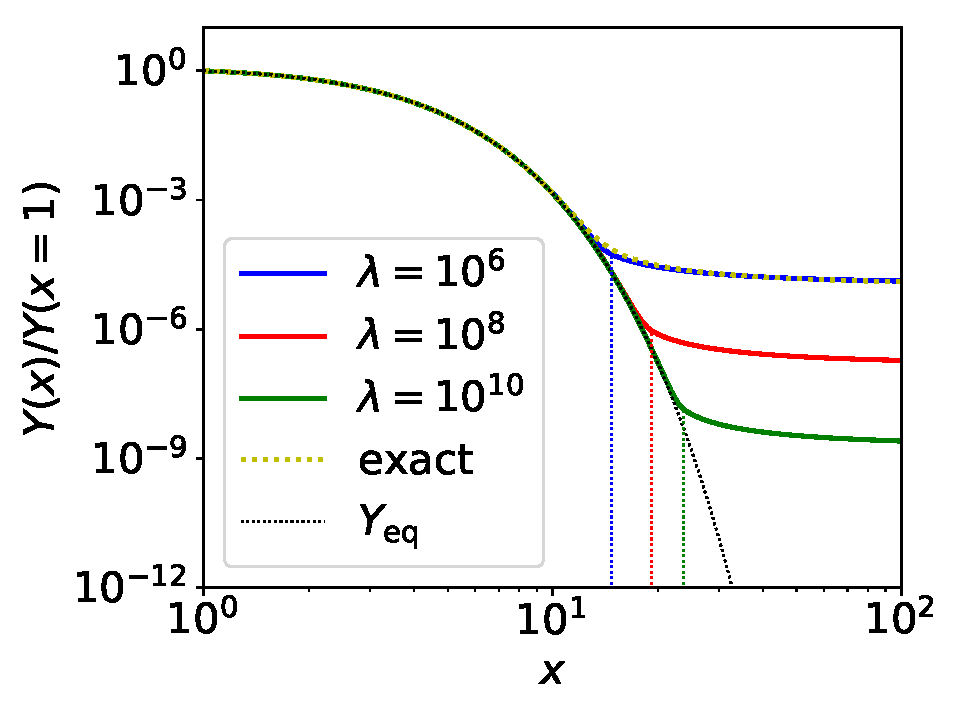
\includegraphics[width=0.5\hsize]{DMrelic.pdf}
  \caption{
    Plot of $Y(x) / Y(x=1)$ with $Y(x)$ being a solution of the evolution equation Eq.~\eqref{eq_boltzmann_Yx}.
    The yellow dotted line is a solution for $\lambda \equiv \left. \Gamma / H \right|_{x=1} = 10^6$, while the black dotted line shows $Y_{\mathrm{eq}} (x) / Y_{\mathrm{eq}} (x=1)$.
    The solid lines are the approximation to the solutions described in the text.
    The blue, red, and green colors correspond to $\lambda = 10^6$, $10^8$, and $10^{10}$, respectively.
    The vertical dotted lines denote the freezeout temperature $x_f$.
  }
  \label{fig_DM_relic}
\end{figure}

Finally, it is known that $\Braket{\sigma v}$ can be expanded as~\cite{Gondolo:1990dk}
\begin{align}
  \Braket{\sigma v} = \Braket{\sigma v}_s +
  \Braket{\sigma v}_p x^{-1} + \cdots,
\end{align}
corresponding to the $s$-wave, $p$-wave, and so on, contributions to the cross section.
When $x \gg 1$, which is the same as the non-relativistic limit, the term with the highest power of $x$ dominates the cross section.  When the $x^{-p}$ term dominates ($p \geq 0$), the temperature dependence of the interaction rate is $\Gamma \propto x^{-3/2-p} e^{-x}$, while the Hubble parameter only reduces as $H \propto \rho^{1/2} \propto x^{-2}$.
As a result, at some point $\Gamma$ becomes smaller than $H$ and $Y$ freezes out as Eq.~\eqref{eq_boltzmann_Yx} indicates.
Hereafter, we focus on the case of the $s$-wave domination with $\Braket{\sigma v}_s \neq 0$ for simplicity.
In Fig.~\ref{fig_DM_relic}, we show the solution of Eq.~\eqref{eq_boltzmann_Yx} for $\lambda \equiv \left. \Gamma / H \right|_{x=1} = 10^6$ by the yellow dotted line.
In the calculation, we use the boundary condition $Y(x=1) = Y_{\mathrm{eq}} (x=1)$ and plot the normalized value $Y(x) / Y(x=1)$.  We also plot the function $Y_{\mathrm{eq}} (x) / Y_{\mathrm{eq}} (x=1)$ by the black dotted line.

Unfortunately, it is computationally hard to solve Eq.~\eqref{eq_boltzmann_Yx} for larger values of $\lambda$ because of the almost complete cancellation between two terms of the right-handed side for small $x\sim \mathcal{O}(1)$ and its amplification caused by large $\lambda$.
We adopt instead to use an approximation that is the same as the one adopted in the public code \texttt{MicrOMEGAs}~\cite{Belanger:2001fz, Belanger:2018mqt}.
For the small $x$ region, the temperature is still high enough to maintain the equilibrium $Y \simeq Y_{\mathrm{eq}}$, which means that $d \Delta Y / d x \ll d Y_{\mathrm{eq}} / d x$ with $\Delta Y \equiv Y - Y_{\mathrm{eq}}$.
From this approximation, we obtain a formula
\begin{align}
  \Delta Y \simeq -\frac{x}{2 \lambda} \frac{d Y_{\mathrm{eq}}}{d x}.\label{eq_relic_app_1}
\end{align}
Then we define the time $x_f$, or equivalently the freezeout temperature $T_f$, when the approximation becomes invalid through the equation\footnote{
  One can easily check that the final relic abundance is not sensitive to the choice of the numerical coefficient $2.5$ in Eq.~\eqref{eq:freezeout_temperature}.
}
\begin{align}
  \Delta Y (x_f) = 2.5 Y_{\mathrm{eq}} (x_f).
  \label{eq:freezeout_temperature}
\end{align}
After the freezeout $x > x_f$, the annihilation of the DM pairs rapidly slows down and the DM abundance far exceeds its equilibrium value: $Y \gg Y_{\mathrm{eq}}$.
Then we can neglect the second term of the right-handed side of Eq.~\eqref{eq_boltzmann_Yx} and obtain the analytical solution
\begin{align}
  Y(x) \simeq - \frac{x}{c_1 x + \lambda / Y_{\mathrm{eq}} (x=1)},\label{eq_relic_app_2}
\end{align}
where $c_1$ is an integration constant.
In Fig.~\ref{fig_DM_relic}, we show results obtained with these two approximations Eqs.~\eqref{eq_relic_app_1} and \eqref{eq_relic_app_2} for $\lambda = 10^6$ (blue), $10^8$ (red), and $10^{10}$ (green).
In particular, the blue and the yellow lines almost completely overlap with each other, which proves the validity of the approximations.
The vertical dotted lines in the figure show the freezeout temperature.
It can be seen from the figure that $x = x_f$ does correspond to the time when $Y$ starts to deviate from $Y_{\mathrm{eq}}$.
Note also that as $\lambda \propto \Braket{\sigma v}$ becomes larger, the freezeout time becomes later and the resulting relic abundance becomes smaller.
It is known that for typical WIMPs with $m_\chi \sim \mathcal{O}(1)\mathrm{TeV}$, $\lambda \sim 10^8$ and thus $T_f \simeq m_\chi / 20$ from the figure.
Then, the freezeout temperature is much larger than the temperature at the radiation-matter equality, and we can confirm that the assumption of the radiation dominated universe at the time of the freezeout is correct.

When the DM properties (\textit{i.e.}, the mass $m_\chi$ and the annihilation cross section $\Braket{\sigma v}$ for a given temperature $T$) are given, corresponding relic abundance can be calculated using above procedure.
In particular, $m_\chi$ determines the normalization of the figure, namely $Y_{\mathrm{eq}} (x=1) = Y_{\mathrm{eq}} (T=m_\chi)$, and $\Braket{\sigma v}$ determines the freezeout temperature through the combination of Eq.~\eqref{eq_lambda}.
Assuming the absence of a non-thermal production, there should be a unique choice of $m_\chi$ corresponding to some $\Braket{\sigma v}$ to explain the current relic abundance of the DM.
From the numerical calculation, we obtain an order estimation formula
\begin{align}
  \Omega_\chi h^2 \sim \frac{3 \times 10^{-27}\,\mathrm{cm^3}/\mathrm{s}}
  {\Braket{\sigma v}_0} \sim
  0.1 \left( \frac{0.01}{\alpha} \right)^2
  \left( \frac{m_\chi}{300\,\mathrm{GeV}} \right)^2,\label{eq_relic_abundance}
\end{align}
where the rough estimation $\Braket{\sigma v} \sim \alpha^2/m_\chi^2$ is used in the last equation with $\alpha$ being the fine structure constant for the DM-SM coupling.
What is fascinating in Eq.~\eqref{eq_relic_abundance} is that a particle can be DM if it has a mass comparable to the electroweak scale and coupling constant comparable to the electroweak coupling constant.
This is the so-called \textit{WIMP miracle}, which supports the hypothesis of the WIMP as a candidate of the DM.
Such $\mathrm{TeV}$-scale WIMPs are theoretically well-motivated in connection with problems of the SM such as the naturalness problem as reviewed in Sec.~\ref{sec:model}.
Also, phenomenologically such $\mathrm{TeV}$-scale WIMPs are of great interest, since they can be detected using several different methods as will be described in this thesis.

In Table \ref{tab:WIMP_property}, we summarize the value of $m_\chi$ for each WIMP model that predicts the correct relic abundance $\Omega_\chi h^2 \sim 0.12$.
As described above, $\mathrm{TeV}$ scale masses are suitable for all WIMP DMs and the required mass becomes larger when we consider a larger $SU(2)_L$ $n$-plet because of the larger annihilation cross section.
However, note that the precise estimation of the relic abundance solely using the last term of Eq.~\eqref{eq_relic_abundance} is not possible, because of the so-called Sommerfeld enhancement effect \cite{Hisano:2004ds,Hisano:2006nn} that may significantly modify the annihilation cross section.
We will review this effect in more detail in Sec.~\ref{sec:indirect_detection} in relation to the indirect detection experiments.
Note also that $m_\chi$ in the table is only an upper bound on the WIMP DM mass because the existence of non-thermal production processes may allow lighter WIMPs to explain the whole relic abundance of DM in the current universe.


%%%%%%%%%%%%%%%%%%%%%%%%%%%%%%%%%%%%%%%%%%%%%%%%%%%%%%%%%%%%%%%%%%%%%%%%%%%%%%%
\subsection{WIMP DM search : direct detection}
\label{sec:direct_detection}
%%%%%%%%%%%%%%%%%%%%%%%%%%%%%%%%%%%%%%%%%%%%%%%%%%%%%%%%%%%%%%%%%%%%%%%%%%%%%%%

There are many experiments aimed at the direct detection of the DM\footnote
{
  For a recent review of the direct detection experiments, see for example \cite{Undagoitia:2015gya}.
}
proposed in \cite{Goodman:1984dc}.
Here, we assume some interaction between the DM and SM particles and look for the recoil of a target SM particle due to the collision with the DM in the laboratory.
In the case of WIMPs of our concern, any particle with non-zero electroweak charges can be a target particle, which interacts with WIMPs through the $t$-channel electroweak gauge boson exchange.
In the traditional setup such as the XENON1T experiment \cite{Aprile:2012zx}, a nucleus (of xenon in XENON1T) and an electron are the frequently used target particles.
From now on, we focus on the nucleus target since, as we will see later, it gives much better sensitivity than the electron target for DMs with a mass of $\mathcal{O} (\mathrm{TeV})$.
In this case, there are several ways to read out the information of the nuclear recoil depending on the deposited energy, such as the use of heat (or photons), an excitation of the nucleus associated with the emission of scintillation light, and the ionization of the atom.
Among them, the XENON1T experiment uses the scintillation light and the ionization.

To evaluate the event rate for this kind of experiment, it is important to know the DM energy density $\rho_0$ and velocity distribution around us.
For this purpose, we model the DM profile in our galaxy using the so-called standard halo model (SHM) and adjust the parameters to the observations.
In the SHM, we assume the DM velocity distribution in the galactic rest frame
\begin{align}
  f(\bm{v}) = \frac{1}{\sqrt{2\pi \sigma}} \exp \left[ -\frac{\bm{v}^2}{2 \sigma^2} \right],
\end{align}
with $\sigma \equiv \sqrt{3/2} v_c$, where $v_c$ denotes the local circular speed of DMs around the Galactic Center.
From the combination of different analyses, we obtain the values $\rho_0 = 0.3\,\mathrm{GeV / cm^3}$ and $v_c = 220\,\mathrm{km/s}$ \cite{Kerr:1986hz,Green:2011bv}.
Also, the DM velocity within the halo cannot be arbitrarily large, since such energetic DM will not be gravitationally bound and will escape from our galaxy.
Correspondingly, we often introduce a cutoff velocity $v_{\mathrm{esc}} = 544\,\mathrm{km / s}$ \cite{Smith:2006ym} and simply assume $f(\bm{v}) = 0$ for $|\bm{v}| > v_{\mathrm{esc}}$.

Using the distribution defined above, the differential event rate per unit recoil energy $E$ per unit material mass is given by \cite{Lewin:1995rx}
\begin{align}
  \frac{d R}{d E} (E,t) = \frac{\rho_0}{m_\chi m_T} \int d^3 v\, v f(\bm{v}, t)
  \frac{d \sigma}{d E} (E, v),
  \label{eq:rate}
\end{align}
where $m_T$ is the mass of the target nucleus, while $d\sigma / dE$ is the differential cross section of the DM-nucleus scattering.
The DM velocity distribution $f(\bm{v}, t)$ is now time-dependent since it represents the distribution observed at the laboratory, which is affected by the motion of the Earth around the Sun and that of the Sun around the Galactic Center.
Thus, $f(\bm{v}, t)$ is derived by performing the Galilean transformation to $f(\bm{v})$ according to the time-dependent velocity of the Earth against the galactic rest frame.
This time-dependence gives the signal a characteristic daily and yearly modulation, which helps us to distinguish it from the background events.
Also, the Galilean transformation makes $f(\bm{v}, t)$ highly anisotropic since the velocity of the Earth is comparable to $v_c$.
Thus, if it is possible to use the directional information, it also helps us to reduce the background.

The differential cross section $d\sigma / dE$, which summarizes the particle physics part of the calculation, is divided into two parts: the spin-independent (SI) part and the spin-dependent (SD) part.
Denoting the SI and SD scattering cross sections for zero momentum transfer as $\sigma_0^{\mathrm{SI}}$ and $\sigma_0^{\mathrm{SD}}$, respectively, we obtain
\begin{align}
  \frac{d\sigma}{d E} (E, v) = \frac{m_T}{2 \mu_T^2 v^2}
  \left( \sigma_0^{\mathrm{SI}} F_{\mathrm{SI}}^2 (E)
  + \sigma_0^{\mathrm{SD}} F_{\mathrm{SD}}^2 (E) \right),
\end{align}
with $\mu_T$ being the reduced mass of the WIMP-nucleus system.
The form factors $F_{\mathrm{SI}}$ and $F_{\mathrm{SD}}$ summarize the nuclear physics part of the matrix element, both of which have properties $F(0)=1$ and $dF / dE < 0$ for large $E$.
Among SI and SD contributions, the SI part is of great interest thanks to the possible coherent enhancement of the cross section.
When the de Broglie wavelength corresponding to the momentum transfer $q$ is longer than the size of the nucleus (corresponding to $q \lesssim 200\,\mathrm{MeV}$ for the xenon), not the individual neutrons and protons but the whole nucleus contribute to the cross section.\footnote{
  When the DM is lighter and the de Broglie wavelength is even longer, the collective excitation modes of nuclei or electrons such as the phonon becomes important (see for example \cite{Knapen:2017xzo}).
  This corresponds to $q \lesssim \mathcal{O}(1)\,\mathrm{keV}$ or $m_\chi \lesssim \mathcal{O}(1)\,\mathrm{MeV}$ and thus we neglect this possibility here.
}
This results in the coherent contribution from all nucleons for the SI case, while only the unpaired nucleons contribute to the cross section for the SD case.
In fact, for the WIMP DM, the SI cross section $\sigma_0^{\mathrm{SI}}$ is enhanced thanks to the coherence by a large factor $A$ that is the mass number of the target nucleus ($A \simeq 130$ for the xenon) as
\begin{align}
  \sigma_0^{\mathrm{SI}} = A^2 \sigma_p^{\mathrm{SI}} \frac{\mu_T^2}{\mu_p^2}
\end{align}
where $\sigma_p^{\mathrm{SI}}$ is the SI scattering cross section for a DM and a single nucleon and $\mu_p$ is the reduced mass of the WIMP-nucleon system.
The above expression dominates over the SD cross contribution for the WIMP DM for most cases.

\begin{figure}[t]
  \centering
  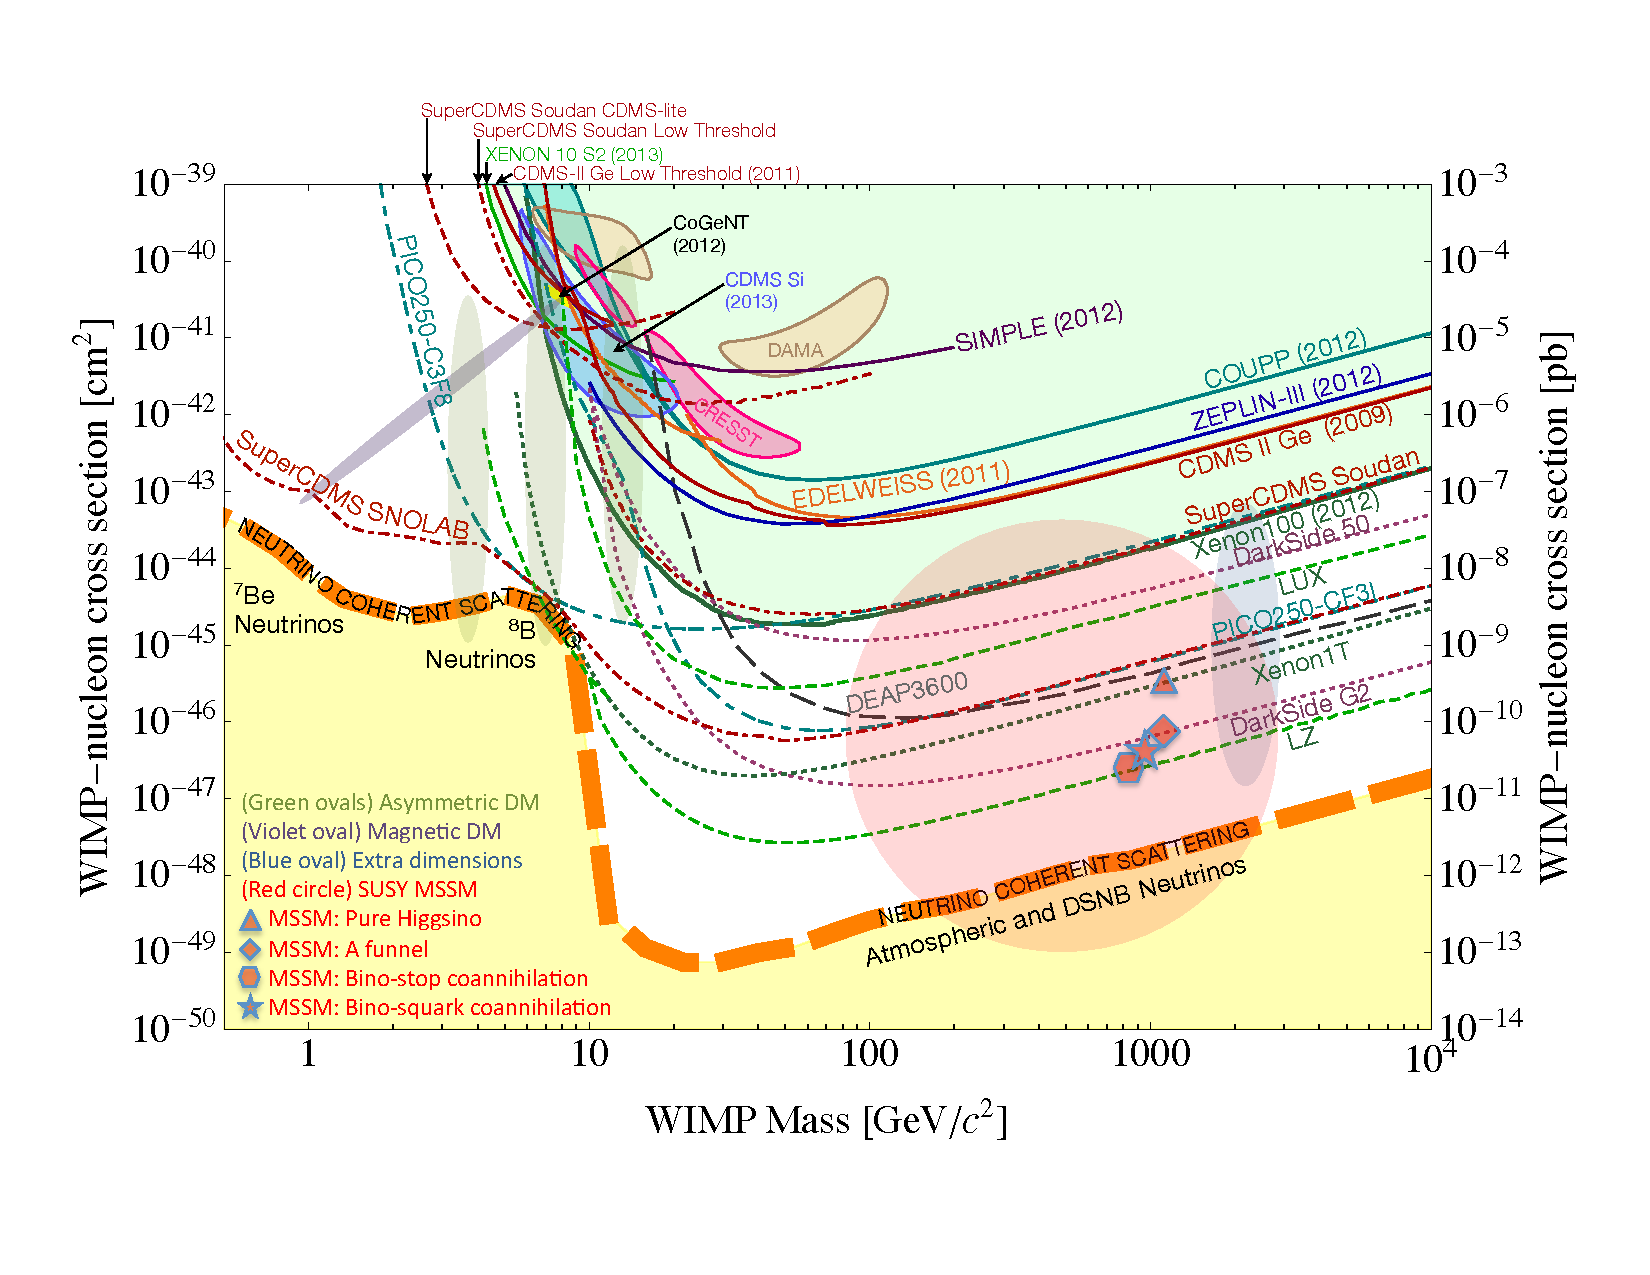
\includegraphics[width=0.8\hsize]{SNOWMASS_LimitPlot_SI_v3.pdf}
  \caption{
    Current constraints and prospects on the DM SI cross section taken from \cite{Cushman:2013zza}.
    The $y$-axis corresponds to $\sigma_p^{\mathrm{SI}}$ in our notation.
  }
  \label{fig:XENON1T}
\end{figure}

In Fig.~\ref{fig:XENON1T}, we show the most recent constraint on the DM SI scattering cross section $\sigma_p^{\mathrm{SI}}$ as a function of its mass.
See \cite{Cushman:2013zza} and references therein for the details of each experiment in the figure.
In the figure, the parameter region above each line is excluded and the yellow region represents the cross section of the background events sourced by neutrinos \cite{Billard:2013qya}.
This background often called as the neutrino floor, which is mainly determined by the solar neutrino for the region $m_\chi \lesssim 10\,\mathrm{GeV}$ and by the atmospheric and supernova neutrinos for $m_\chi \gtrsim 10\,\mathrm{GeV}$, roughly represents the maximum possible sensitivity of the direct detection method.\footnote{
  It may be possible, in particular for the solar neutrino background, to significantly reduce the number of background events and go beyond the neutrino floor by using the directional information of the signals.
}
Currently, the XENON1T collaboration~\cite{Aprile:2018dbl} provides the most stringent constraint in the (sub-)$\text{TeV}$ region of our interest.
Prospects of future planned experiments called DarkSide G2 \cite{Aalseth:2015mba} and LZ \cite{Mount:2017qzi} are also shown in the figure.

The qualitative description of the form of the sensitivity curve in Fig.~\ref{fig:XENON1T} can be given using the above discussion.
The sensitivity for a very light WIMP is weak because of the finite threshold $E_{\mathrm{thr}}$ of the recoil energy required for the detection of the signal.
The threshold effect can be taken into account by choosing the lower boundary of the $\bm{v}$-integral in Eq.~\eqref{eq:rate} to be $v_{\mathrm{min}}$ defined as
\begin{align}
  v_{\mathrm{min}} = \sqrt{\frac{m_T E_{\mathrm{thr}}}{2 \mu_T^2}}.
\end{align}
Since $v_{\mathrm{min}} \propto m_\chi^{-1}$ for $m_\chi \ll m_T$, the event rate rapidly becomes smaller for smaller $m_\chi$.
On the other hand, heavier WIMP DMs have less number density with the energy density $\rho_0$ fixed.
Because of this, the sensitivity for a heavy WIMP becomes moderately worse when $m_\chi$ increases.
These two behaviors determine the best suitable $m_\chi$ for each choice of $m_T$ and $E_{\mathrm{thr}}$, which is the reason why the xenon nucleus target is more suitable for the $\mathrm{TeV}$-scale WIMP search than the electron target.
The latter choice is suitable when we search for lighter DMs.

Although no signal of DM is observed yet, this null result is still consistent with WIMP models of our concern.
For example, the Wino DM scatters with a nucleon through the t-channel exchange of a higgs boson or two $W$ gauge bosons at the one-loop order or higher.
The calculation of the scattering cross section up to the next-to-leading order in $\alpha_s$ reveals that it almost mass-independently takes a small value of $\sigma_p^{\mathrm{SI}} \simeq 2.3 \times 10^{-47}\,\mathrm{cm}^2$~\cite{Hisano:2015rsa}, which is below the current constraint but is a region of future interest.
As for the MDM, the $5$-plet fermion is analyzed in \cite{Hisano:2011cs} and the scattering cross section $\sigma_p^{\mathrm{SI}} \simeq 10^{-46}\,\mathrm{cm}^2$ is obtained.
However, the mass requirement $m_\chi \sim 10\,\mathrm{TeV}$ (see Table~\ref{tab:WIMP_property}) makes the detection difficult and the sensitivity will not cover the whole region of the viable parameter space.
In general, a pure $SU(2)_L$ multiplet with non-zero hypercharge has a large contribution to $\sigma_p^{\mathrm{SI}}$ from the tree-level exchange of $Z$ boson \cite{Farina:2013mla}.
Thus, for such a particle to be a viable DM candidate, we should modify the model to forbid the tree-level scattering.
Related to this point, the Higgsino-like DM is a kind of a mixed multiplet that can avoid the tree-level scattering via $Z$ boson.
As is discussed in Sec.~\ref{sec:mass_splitting}, the mixing between Higgsino and gauginos splits the masses of two neutral components of the Higgsino-like state, making them two Majorana fermions.
As a result, the neutral components have vanishing interaction with $Z$ boson and loop-suppressed scattering cross section for the direct detection dominates.
The constraint on the Higgsino-like state is highly model-dependent since the size of the mixing significantly modifies the scattering cross section.
According to \cite{Hisano:2012wm, Roszkowski:2014wqa}, the almost pure Higgsino has $\sigma_p^{\mathrm{SI}}$ below the neutrino floor, while some of the parameter space with a sizable mixing has much larger $\sigma_p^{\mathrm{SI}}$ that is already excluded.
Thus, we conclude that the almost pure Higgsino is difficult to search for using this method.


%%%%%%%%%%%%%%%%%%%%%%%%%%%%%%%%%%%%%%%%%%%%%%%%%%%%%%%%%%%%%%%%%%%%%%%%%%%%%%%
\subsection{WIMP DM search : indirect detection}
\label{sec:indirect_detection}
%%%%%%%%%%%%%%%%%%%%%%%%%%%%%%%%%%%%%%%%%%%%%%%%%%%%%%%%%%%%%%%%%%%%%%%%%%%%%%%

The indirect detection of DM\footnote{
  For a recent review of the indirect detection experiments, see for example \cite{Gaskins:2016cha}.
}
uses the DM annihilation process into SM particles to detect the DM signal.
When DM is composed of WIMPs, their annihilation can be again explained by the electroweak interaction.
Since DMs are non-relativistic in the current universe, the $s$-wave contribution to the annihilation cross section, if exists, dominates over others, which results in the dominant annihilation process coming from the $t$- and $u$-channel exchange of a virtual WIMP.
Then, some of the final state particles may propagate to the earth and be observed by telescopes in the form of gamma-rays, neutrinos, cosmic rays, and so on.

The DM annihilation rate at some point $\bm{x}$ of the universe has a quadratic dependence on the local DM energy density $\rho_\chi (\bm{x})$.\footnote{
  More precisely, the annihilation rate has a quadratic dependence on the DM number density $n_\chi (\bm{x})$.
  This means that, for some fixed value of $\rho_\chi (\bm{x})$, the lighter DM has more chance to annihilate since $n_\chi = \rho_\chi / m_\chi$.
}
In our case, we focus on the photons produced at the WIMP annihilation, and the main targets of indirect detection experiments are the center of galaxies or galaxy clusters, where abundant DM is expected to be accumulated thanks to the strong gravitational potential.
The DM energy density distribution around each galaxy (cluster) can be determined by the observation of the rotation curve of luminous objects.
One of the model functions introduced to fit such observations is the so-called the Navarro-Frenk-White (NFW) profile \cite{Navarro:1995iw, Navarro:1996gj} of the DM density distribution,
\begin{align}
  \rho_{\mathrm{NFW}} (r) = \frac{\rho_s}
  { \left( \frac{r}{r_s} \right) \left[ 1 + \left( \frac{r}{r_s} \right) \right]^2},
\end{align}
where $r$ is the distance from the center of the galaxy of our concern.
Free parameters $\rho_s$ and $r_s$ should be chosen to fit the data for each galaxy, which gives for our galaxy $\rho_s \sim 1\times 10^7 M_\odot\, \mathrm{kpc}^{-3}$ and $r_s \sim 20\,\mathrm{kpc}$ \cite{Fornasa:2013iaa} with $M_\odot$ being the solar mass.

\begin{figure}
  \centering
  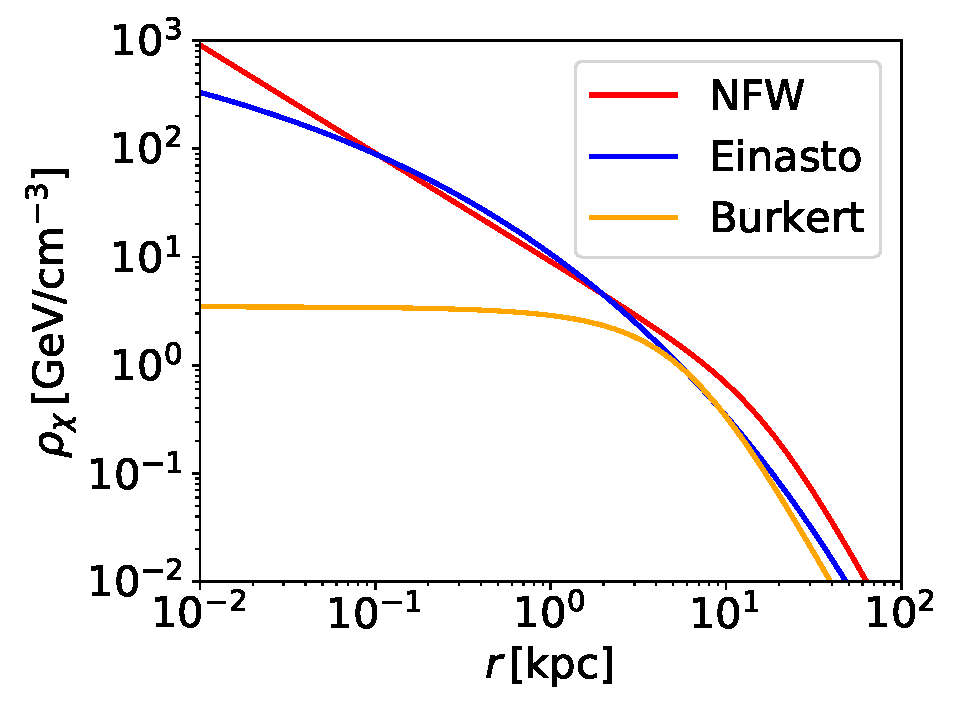
\includegraphics[width=0.5\hsize]{profile.pdf}
  \caption{
    Dark matter energy density $\rho_\chi$ within our galaxy as a function of the distance from the galactic center $r$.
  }
  \label{fig:profile}
\end{figure}

The inner slope of the NFW profile follows $\rho_{\mathrm{NFW}} \propto r^{-1}$.
On the other hand, many observations of the rotation curve and models of dwarf galaxies suggest the scaling behavior $\rho \propto r^0$, which is the so-called core-cusp problem (see \cite{Genina_2017} and references therein).
To take account of this behavior, other profiles are also widely used: the Einasto profile \cite{1965TrAlm...5...87E, Graham:2005xx}
\begin{align}
  \rho_{\mathrm{Einasto}} (r) = \rho_s \exp \left[
  -\frac{2}{\alpha} \left\{ \left( \frac{r}{r_s} \right)^\alpha - 1 \right\} \right],
\end{align}
with $\rho_s \sim 5 \times 10^6 M_\odot\, \mathrm{kpc}^{-3}$, $\alpha \sim 0.2$, and $r_s \sim 10\,\mathrm{kpc}$ for our galaxy, and the Burkert profile \cite{Burkert:1995yz}
\begin{align}
  \rho_{\mathrm{Burkert}} (r) = \frac{\rho_s}
  {\left( 1 + \frac{r}{r_s} \right) \left( 1 + \frac{r^2}{r_s^2} \right)},
\end{align}
with $\rho_s \sim 9 \times 10^7 M_\odot\, \mathrm{kpc}^{-3}$ and $r_s \sim 6\, \mathrm{kpc}$ for our galaxy.
In Fig.~\ref{fig:profile}, we show the DM energy density distribution in our galaxy.\footnote{
  In principle, all the profiles should reconstruct the DM density at the Sun $\rho (r \sim 8\, \mathrm{kpc}) \sim 0.3\, \mathrm{GeV} / \mathrm{cm}^3$, which is apparently not the case.
  This deviation can be explained by the effect of the fitting error, which results in an order of magnitude uncertainty in $\rho_\chi$ at the $68\,\%$ level.
}
As for the choice of parameters, we use the mean values of fits of several observations listed in \cite{Fornasa:2013iaa}.
We can see the difference in shapes among three profiles at the small $r$ region.

Next we derive the formula to estimate the event rate of the indirect detection experiments.
The event rate at the laboratory can be divided into the particle physics part and the astrophysical part, the second of which, referred to as the $J$-factor, is related to the DM density distribution.
The $J$-factor for the DM annihilation for a sky patch with solid angle $\Delta\Omega$ around a sky direction $\hat{\bm{n}}$ is given by
\begin{align}
  J(\hat{\bm{n}}, \Delta\Omega) = \int_{\Omega \sim \hat{\bm{n}}} d\Omega
  \int_{\mathrm{LOS}} \rho_\chi^2 (\Omega, \ell) d\ell,
  \label{eq:J-factor}
\end{align}
where $\ell$ is a distance along the line-of-sight (LOS) defined by the direction $\Omega$.
The first integration performed over a region $\Delta\Omega$ around the direction $\hat{\bm{n}}$, while the second one sums up all the contributions from DMs on the LOS.
Using this, the flux $\Phi_x(E, \hat{\bm{n}}, \Delta\Omega)$ of a SM particle $x$ with energy $E$ at the sky patch is expressed as\footnote{
  We identify the DM particle and anti-particle in the calculation of Eq.~\eqref{eq:flux}.
  If this is not the case, the right-handed side should be multiplied by an extra factor of $1/2$.
}
\begin{align}
  \Phi_x (E, \hat{\bm{n}}, \Delta\Omega) = \frac{\Braket{\sigma v}}{8\pi m_\chi^2}
  \frac{d N_x}{d E} J(\hat{\bm{n}}, \Delta\Omega),
  \label{eq:flux}
\end{align}
where $\Braket{\sigma v}$ and $d N_x / d E$ are the thermally averaged DM annihilation cross section and the differential spectrum of $x$ per annihilation, respectively.

\begin{table}[t]
  \centering
  \begin{tabular}{c|c}
    Target & $\log_{10} (J(\hat{\bm{n}}, \Delta\Omega) / \mathrm{GeV}^2 \mathrm{cm}^{-5})$ \\ \hline
    Galactic Center & 21.5\\
    Dwarf Galaxies & 16--19\\
    Galaxy clusters & $\sim 20$
  \end{tabular}
  \caption{Comparison of $J$-factors for several targets of DM indirect detection.}
  \label{tab:J-factors}
\end{table}

In Table \ref{tab:J-factors}, we summarize $J$-factors for several astrophysical targets suitable for the indirect detection of DM.
Values are taken from \cite{Fornasa:2013iaa, Geringer-Sameth:2014yza, S_nchez_Conde_2011}.
We show the result with $\hat{\bm{n}}$ and $\Delta\Omega$ being the direction of the target and the size of the target observed from the earth, respectively.\footnote{
  In \cite{S_nchez_Conde_2011}, the authors use a different definition of the $J$-factor
  \begin{align}
    J_T \equiv \frac{1}{4\pi D^2} \int dV \rho_\chi^2,
  \end{align}
  where $D$ is the distance from the earth to the target, while the integral is performed over the whole volume of the target.
  This definition possesses an advantage especially for the assumption of the NFW profile, which becomes ill-defined around the center of the target in the integration process in Eq.~\eqref{eq:J-factor}.
  Due to this difference, it is difficult to convert the $J$-factor of their definition calculated with the NFW profile into that of our definition, and the result of the rough estimation is shown in the table.
}
In the table, the results for the center of our galaxy, $20$ dwarf galaxies in our galaxy, and $7$ galaxy clusters are shown.
Among the targets listed in the table, the Galactic Center seems to be the best source for indirect detection, which however suffers from huge background events at the same time.
Dwarf galaxies may be a more promising target since it provides much cleaner signals and the combined analysis of several targets can be performed to enlarge the statistics.
Galaxy clusters may also be an interesting target since its power for the DM detection strongly depends on the DM profile of each galaxy cluster and a large enhancement may be expected for clusters that have relatively cusped DM profiles for some reason.

\begin{figure}[t]
  \centering
  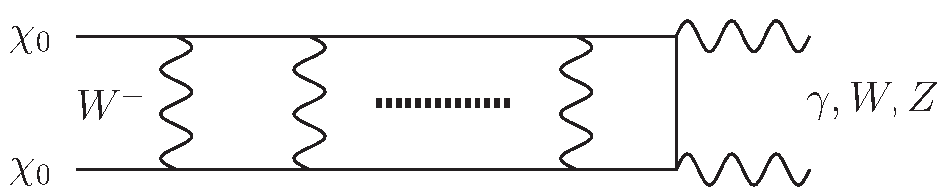
\includegraphics[width=0.7\hsize]{Sommerfeld.pdf}
  \caption{Ladder diagram contribution to the DM annihilation.}
  \label{fig:ladder}
\end{figure}

There remains a missing piece to describe the phenomenology of $\mathrm{TeV}$-scale DMs: the Sommerfeld enhancement effect \cite{Hisano:2004ds, Hisano:2006nn}.
This effect becomes important when the DM particles become non-relativistic like those in the current universe.
Consider the repeated exchange of electroweak gauge bosons between two initial DM particles before the annihilation as shown in Fig.~\ref{fig:ladder}, which is sometimes called a ladder diagram.
At a glance, the contribution of this diagram seems to be suppressed compared with the tree-level annihilation by a factor of $(\alpha/4\pi)^n$, where $\alpha \sim \alpha_1 \sim \alpha_2$ is a typical size of the coupling and $n$ is the number of gauge boson exchange.
However, when the initial particles are non-relativistic, it turns out that the proper power counting should be something like $(\alpha/\beta)^n$ instead of $\alpha^n$, where $\beta$ is the velocity of initial particles, observed in the center-of-mass system for simplicity.
This results in a possibly large contribution from ladder diagrams and we need to resum all of them to calculate the annihilation cross section accurately.
This effect affects both the thermal relic abundance of DM and the event rate at the indirect detection experiments, but the effect on the latter is typically larger since the average value of $\beta$ is smaller in the current universe than that at the freezeout temperature.

The resummation procedure can be performed by the use of the Bethe-Salpeter equation \cite{Salpeter:1951sz} as in \cite{Strassler:1990nw}.
Or equivalently, this effect can be seen as the deformation of the two-DM wave function from the plane wave according to the potential energy between them sourced by the electroweak interaction.
In this viewpoint, it is intuitive that the physics can be described by the Schr\"{o}dinger equation
\begin{align}
  \left[ - \frac{1}{m_\chi} \frac{d^2}{d r^2} + V(r) \right] \psi = E \psi,
\end{align}
where $\psi(r)$ is the s-wave part of the two-DM wave function, $r$ is the distance between two DMs, and $V(r)$ and $E = m_\chi \beta^2$ are the potential and kinetic energies of the two DM system, respectively.
Besides, we impose the outgoing boundary condition
\begin{align}
  \psi(r) \to e^{i p r} ~~ (r \to \infty),
\end{align}
with $p = m_\chi \beta$ being the DM momentum.
Remembering that the DM-DM interaction is local, the Sommerfeld enhancement factor $R$ that multiplies the tree-level cross section is given by $R = \left| \psi(\infty) / \psi(0) \right|^2$.
For example, when we consider the Coulomb potential $V(r) = -\alpha / r$, the equation can be analytically solved and we obtain
\begin{align}
  R = \frac{\pi \alpha / \beta}{1 - e^{- \pi \alpha / \beta}},
\end{align}
which causes a huge enhancement of the cross section when $\beta$ is small and $\alpha > 0$, or equivalently, the force between DMs is attractive.

The problem possesses an interesting feature when we consider a potential that is non-negligible only for a finite range such as the Yukawa potential for the electroweak interaction $V(r) = \alpha_2 e^{-m_W r} / r$.
In this case, when we neglect the small mass difference among an $SU(2)$ multiplet, the factor $R$ is strongly enhanced when the initial particle mass satisfies the equation
\begin{align}
  \sqrt{2} p_c = (2n - 1) \frac{\pi}{2}~~(n = 1, 2, \dots),
\end{align}
with $p_c \equiv \sqrt{2 \alpha_2 m_\chi / m_W}$.\footnote{
  If the mass difference $\delta m$ among an $SU(2)_L$ multiplet is comparable or larger than $\alpha_2 m_W$, the peaks move to the heavier direction.
  This may be the case for Higgsinos with a large mixing with gauginos.
}
Each choice of $n$ corresponds to a model point that has a bound state with zero binding energy and the enhancement is called the zero-energy resonance \cite{Landau1981Quantum}.
Note that the first peak with $n=1$ corresponds to $m_\chi \sim 2\,\mathrm{TeV}$, which is compatible with the assumption of the Wino DM or the MDM with the help of the non-thermal production.
Accordingly, as we will see from now, small regions around peaks of such models have already been excluded by the indirect detection experiments.

\begin{figure}[t]
  \centering
  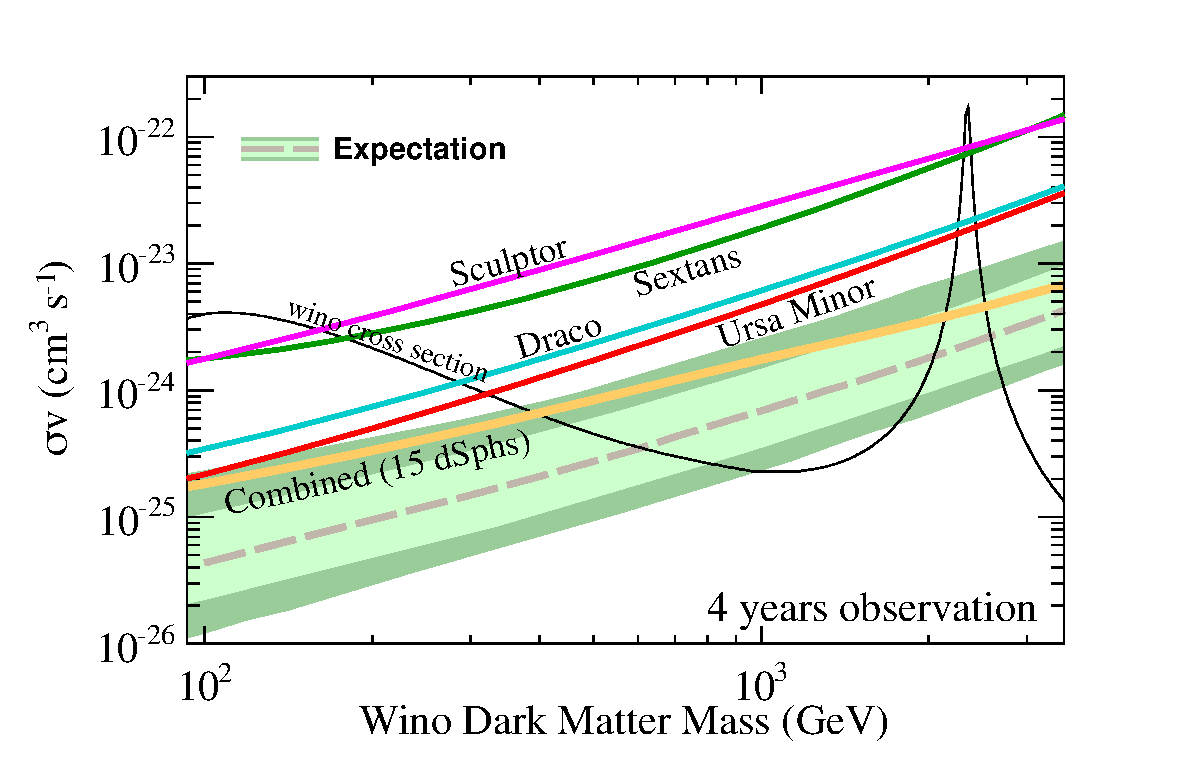
\includegraphics[width=0.6\hsize]{Present_limit.pdf}
  \caption{
    Constraint at the $95\,\%$ confidence level on the DM annihilation cross section taken from \cite{Bhattacherjee:2014dya}.
    The gray dotted line shows the combined result of $4$ years observation of $15$ dwarf galaxies by the Fermi-LAT collaboration, and the green bands show the observational errors.
    For the calculation of the constraint, the NFW profile is used.
    Also shown in the black solid line is the annihilation cross section of Wino.
  }
  \label{fig:indirect_current}
\end{figure}

There are many astrophysical observations that focus on several different particles or photons with different wavelengths.
Among them, the most stringent bound on DMs comes from the gamma-ray observations provided by several currently working or future planned collaborations such as the Fermi-LAT \cite{Atwood_2009}, GAMMA-400 \cite{GALPER2013297}, H.E.S.S. \cite{Abdallah:2016ygi}, and CTA \cite{Carr:2015hta}.
For Wino DM, for example, the annihilation mode into $W^{+} W^{-}$ dominates over the other modes and the photons emitted associated with the $W$-boson decay will be observed.
In Fig.~\ref{fig:indirect_current}, we show the constraint at the $95\,\%$ confidence level on the DM annihilation cross section, assuming $100\,\%$ branching ratio into $W^{+} W^{-}$ \cite{Bhattacherjee:2014dya}.
The gray dotted line shows the combined result of $4$-year observation of $15$ dwarf galaxies by the Fermi-LAT collaboration, while the black solid line denotes the annihilation cross section of Wino.
Note the existence of the zero-energy resonance at the position of $m_\chi \sim 2\,\mathrm{TeV}$ as estimated above.
From the figure, we can see that the parameter regions of Wino DM $m_\chi \lesssim 400\,\mathrm{GeV}$ and $m_\chi \sim 2\,\mathrm{TeV}$ are already excluded.\footnote{
  Currently, almost $10$-year observation data is expected to be accumulated and no sign of DM is reported.
  According to the estimation in \cite{Bhattacherjee:2014dya}, this may correspond to the exclusion of $m_\chi \lesssim 800\,\mathrm{GeV}$ and a slightly larger range around $m_\chi \sim 2\,\mathrm{TeV}$.
}

A similar analysis can be performed for other WIMP DM candidates.
The Higgsino is currently constrained only up to $350\,\mathrm{GeV}$ \cite{Krall:2017xij} due to the smallness of the annihilation cross section in particular for the heavier region.
For the MDM, 5-plet fermion is analyzed as an example in \cite{Abdalla:2018mve} and $m_\chi \lesssim 2\,\mathrm{TeV}$ and several narrow regions corresponding to the resonances are excluded.
As for the prospects of future experiments, firstly, an order of magnitude improvement on the constraint from that shown in Fig.~\ref{fig:indirect_current} is expected \cite{Bhattacherjee:2014dya} by a combination of the $15$-year observation at the Fermi-LAT and the $10$-year observation at the GAMMA-400, which covers most of the allowed parameter region of Wino DM.
Besides, the observation of the Galactic Center at the CTA collaboration will probe the relatively heavier region $m_\chi \sim \mathcal{O}(1)\, \mathrm{TeV}$ efficiently, reaching $\sigma v \sim \text{(a few)} \times 10^{-26}\, \mathrm{cm^3\, s^{-1}}$.
However, note that the observation of the Galactic Center is highly sensitive to the astrophysical uncertainties such as those on the $J$-factor.
Note also that the thermal Higgsino DM may be a challenging target of this kind of experiment even in the future, whose mass and cross section are $m_\chi \sim 1\,\mathrm{TeV}$ and $\sigma v < 10^{-26}\, \mathrm{cm^3\, s^{-1}}$, respectively.


%%%%%%%%%%%%%%%%%%%%%%%%%%%%%%%%%%%%%%%%%%%%%%%%%%%%%%%%%%%%%%%%%%%%%%%%%%%%%%%
\subsection{Concluding remarks}
\label{sec:summary_DM}
%%%%%%%%%%%%%%%%%%%%%%%%%%%%%%%%%%%%%%%%%%%%%%%%%%%%%%%%%%%%%%%%%%%%%%%%%%%%%%%

In this section, we have described the possibility of WIMPs to be the dominant component of DM.
We have seen that the $\mathrm{TeV}$-scale WIMPs with electroweak interactions can explain the DM relic abundance and studied two search methods of such WIMP DMs.
Both direct and indirect detection have strong powers to explore a large region of the WIMP mass.
However, it is revealed that the almost pure Higgsino will be difficult to probe because of its small scattering and annihilation cross section.
Besides, the constraints shown above assume the whole DM is composed of a WIMP and are also sensitive to the possibly large astrophysical uncertainties.
From the next section, we will see more robust ways of the WIMP search using collider experiments and consider whether we can probe the regions of the parameter space that are difficult to probe using DM search experiments.


\bibliographystyle{elsarticle-num}
\bibliography{../phd}

\end{document}
